\section{The collision of the two opposite mindsets: Innovation and Entrepreneurship
in China and Switzerland}

\subsection{Switzerland is an old friend of China}

Switzerland had significant economic interests in China at the time, especially
in Shanghai. The prompt recognition of the new communist government, as well
as Switzerland's status as a neutral country, allowed it to gain political
advantage and carve out a role as mediator in the region.

On October 7, 1949, the Federal Coucil (Swiss executive branch) had already
decided to recognise the Chinese government, in order to avoid being "either
one of the first or the last" to do so.

The official recognition came on January 17, 1950. Of the Western nations,
only Great Britain and Scandinavian countries were earlier in doing so.

The two countries formally established diplomatic relations on September
14 in the same year.

\vspace{1\baselineskip}

In the 1970s, the good Swiss-Chinese relations revolved mainly around the hope
that the Swiss economy might benefit from the future opening of the Chinese
market to external commerce. And indeed, in December 1974, Bern and Beijing
signed a trade deal - and then a free trade agreement 40 years later.

\begin{figure}[h]
    \centering
    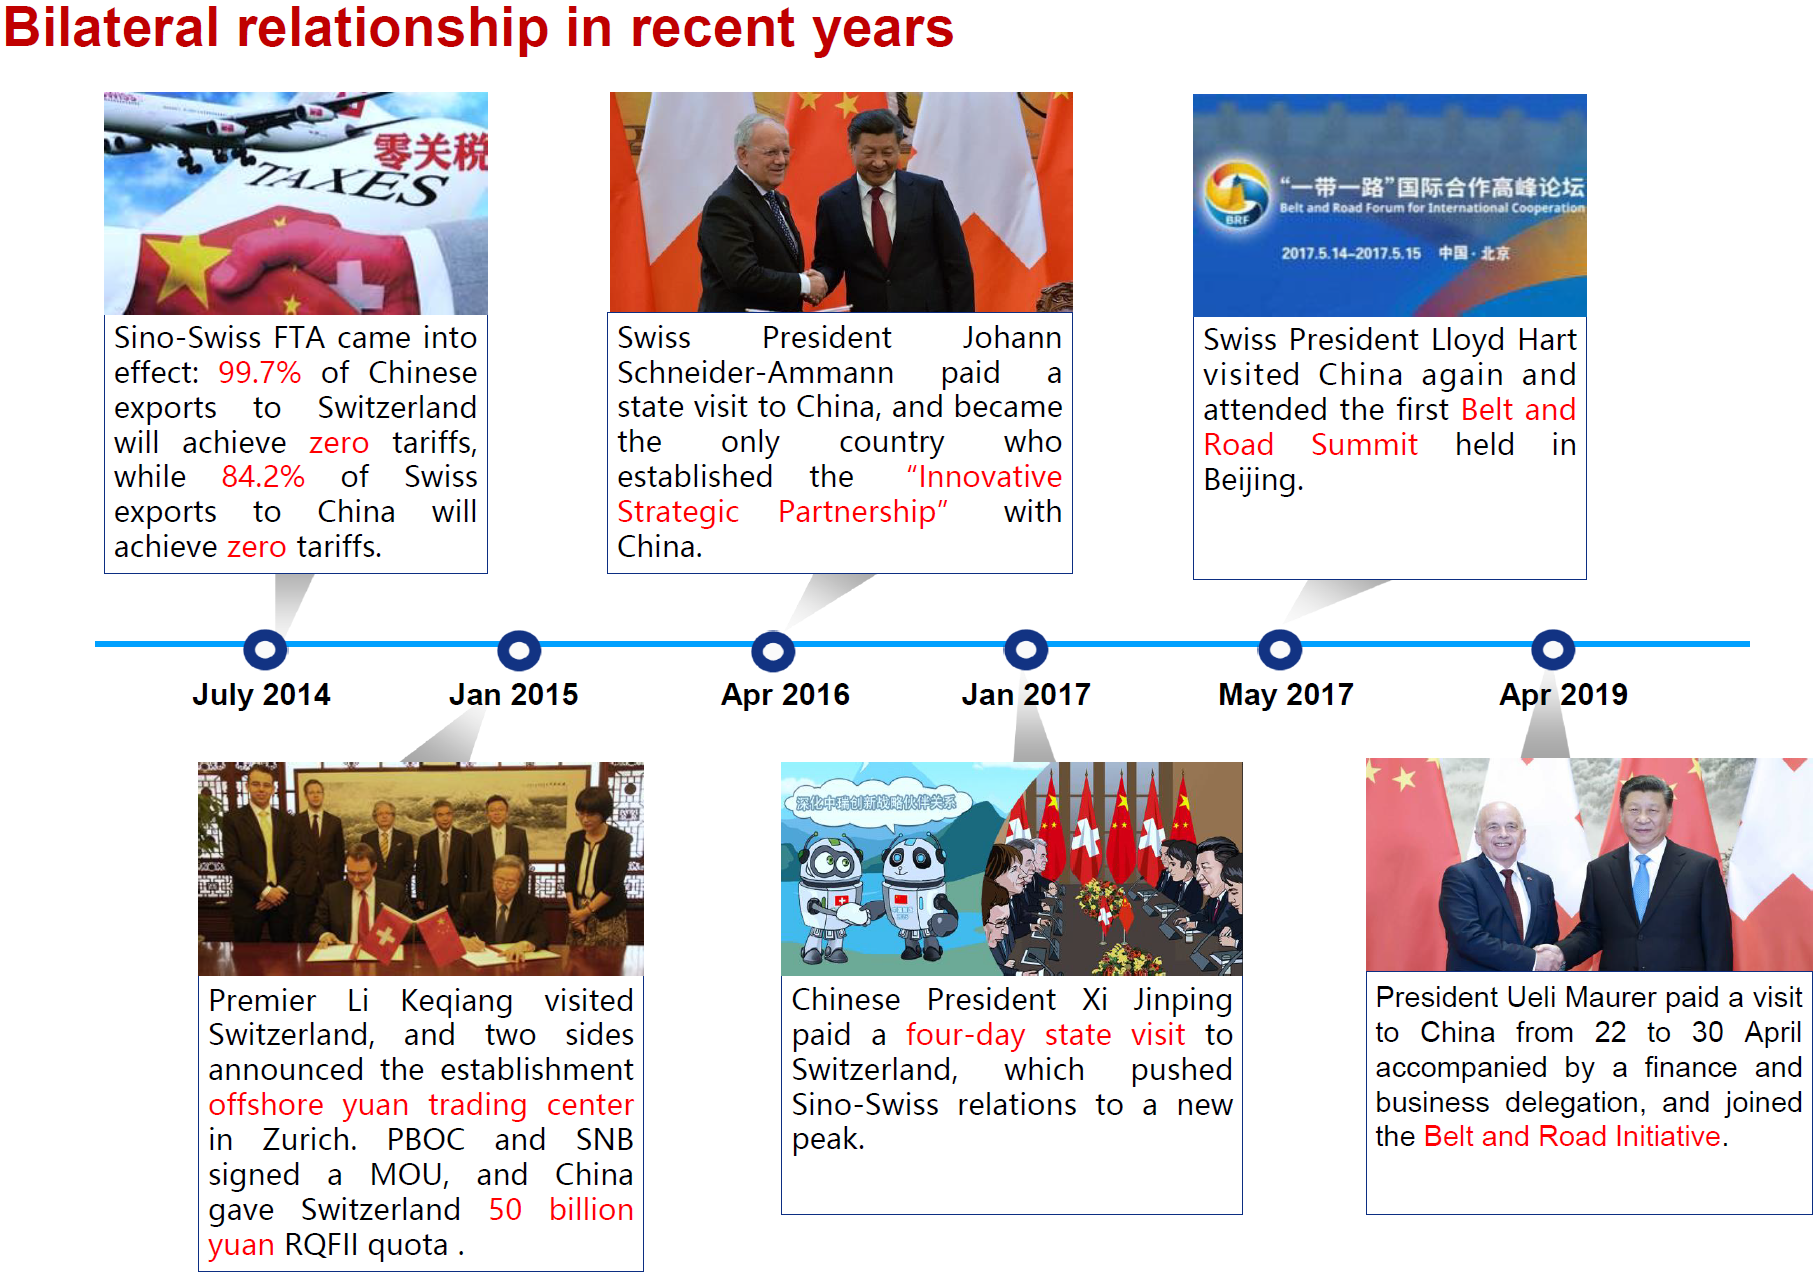
\includegraphics[width=0.8\textwidth]{Pictures/bilateral_china_switzerland.png}
\end{figure}

\begin{itemize}
    \item Switzerland has also strenghened financial ties with China over the
        years. In December 2018, UBS became the first foreign bank to gain
        majority control of a financial institution on mainland China by increasing
        its stake in the UBS Security joint venture to 51\%.
    \item In 2016, the China Construction Bank (CCB) became the first Chinese
        bank to open a branch on Swiss soil. CCB was followed by the Industrial
        and Commercial Bank of China a year later. The development has cemented
        Switzerland's positoin as a renminbi trading hub.
    \item A latent trade war currently exists between China and several Western
        countries, notably the US. Not with Switzerland though. Sino-Swiss
        economic ties were deepene by a free-trade agreement external link
        (FTA) that came into force on July 1, 2014. This is one of the few FTAs
        that China has signed external link with countries outside the
        Asia-Pacific region.
    \item Billed to save Swiss companies CHF 290 million annually by the time all
        trade barriers are lifted in 2023, a study last year found the FTA
        had achieved savings of CHF 100 million for both Swiss and Chinese
        firms in 2017.
    \item More than 80 Swiss companies are now in Chinese hands, with a total
        value of CHF 46 billion. The \$43.3-billion takeover of agrochemical
        giant Syngenta by the China National Chemical Corporation (ChemChina)
        in 2016 is the biggest acquisition ever by a Chinese company.
\end{itemize}

\paragraph{Import and Export:}

\begin{itemize}
    \item Export elasticity can be used to determine the effects of a sharp
        decline in China's growth on Swiss exports. Under the assumption of
        a constant exchange rate, export elasticity shows by how many
        percentage points the exchange growth in Switzerland would increase
        or decrease if the growth of China's GDP changes by one percentage
        point.
    \item The elasticity between Switzerland and China is not statistically
        significant. However, when you look at individual industries, you
        see that, at 2.6 percent points, the food industry in particular
        is very dependent on China's economic situation. The watch and
        machinery industries are also expecially sensitive to changes in
        the Chinese economy.
    \item Switzerland exports mainly finished products, so the Swiss economy
        is particularly dependent on Chinese final demand.
    \item Swiss exports to Germany are also influenced by China's economic
        development, as 20\% of exports to Germany are processed there and then
        exported to China, among other countries. One prominent example
        of this is the automotive industry.
\end{itemize}

\begin{figure}[H]
    \centering
    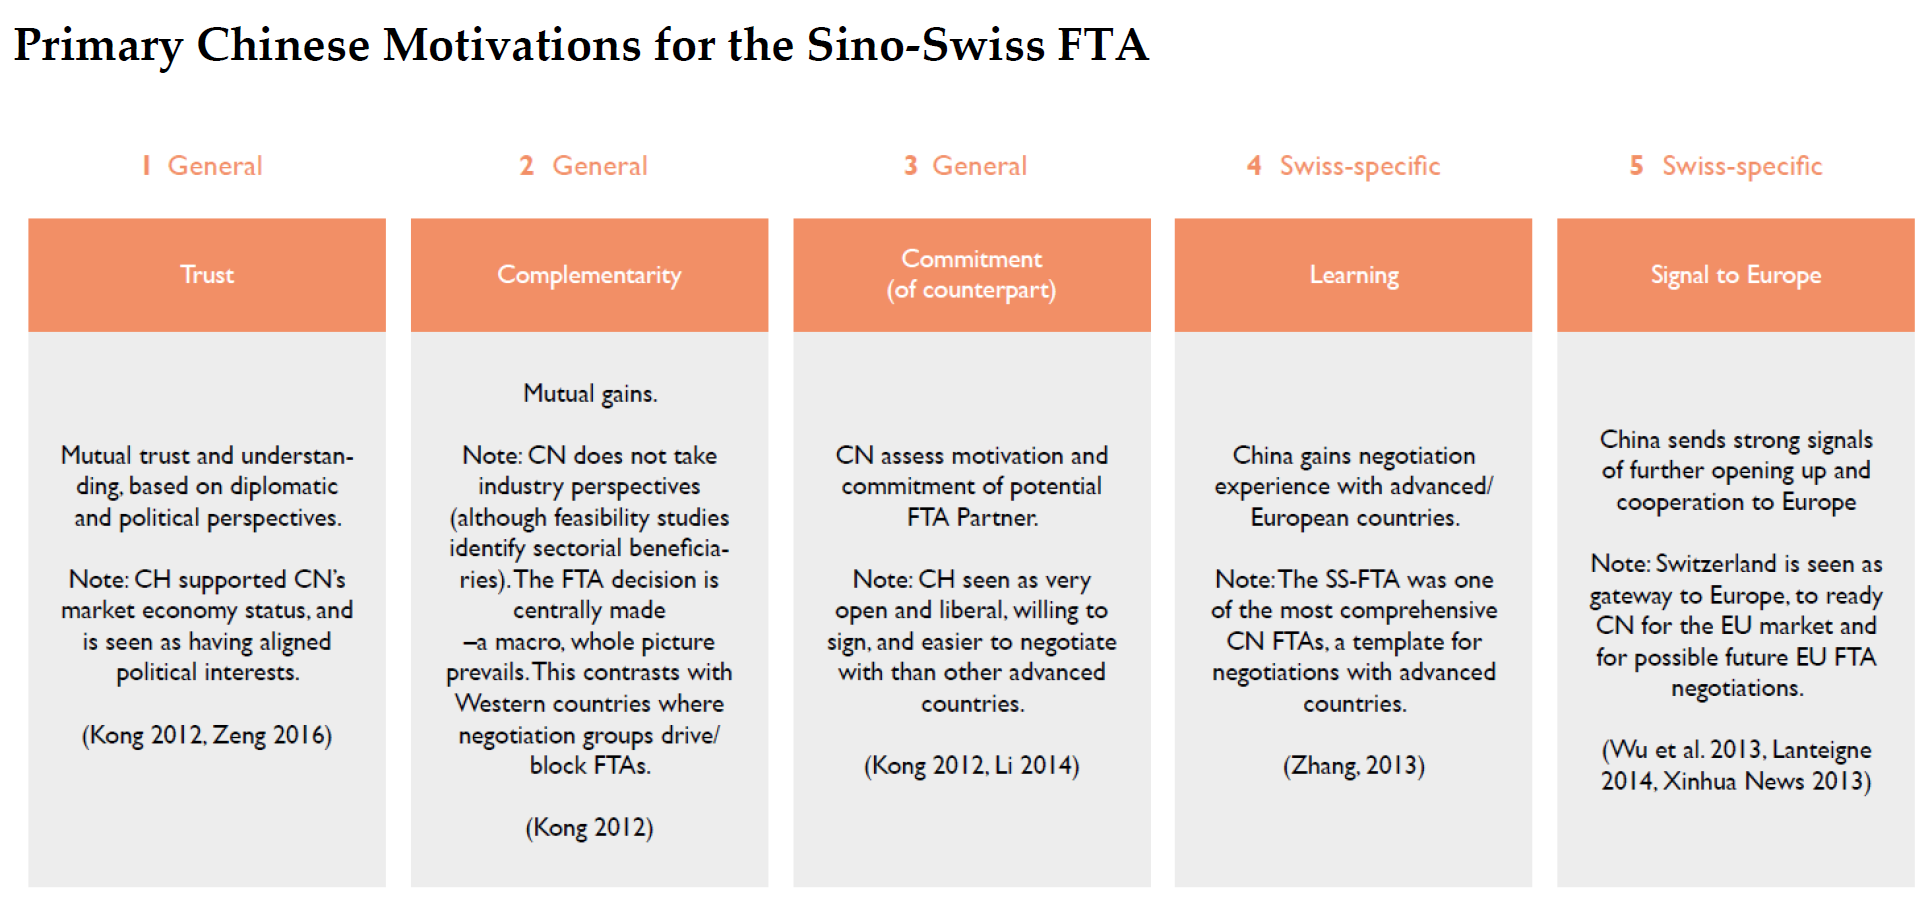
\includegraphics[width=0.9\textwidth]{Pictures/chinese_motivation.png}
\end{figure}

\begin{figure}[H]
    \centering
    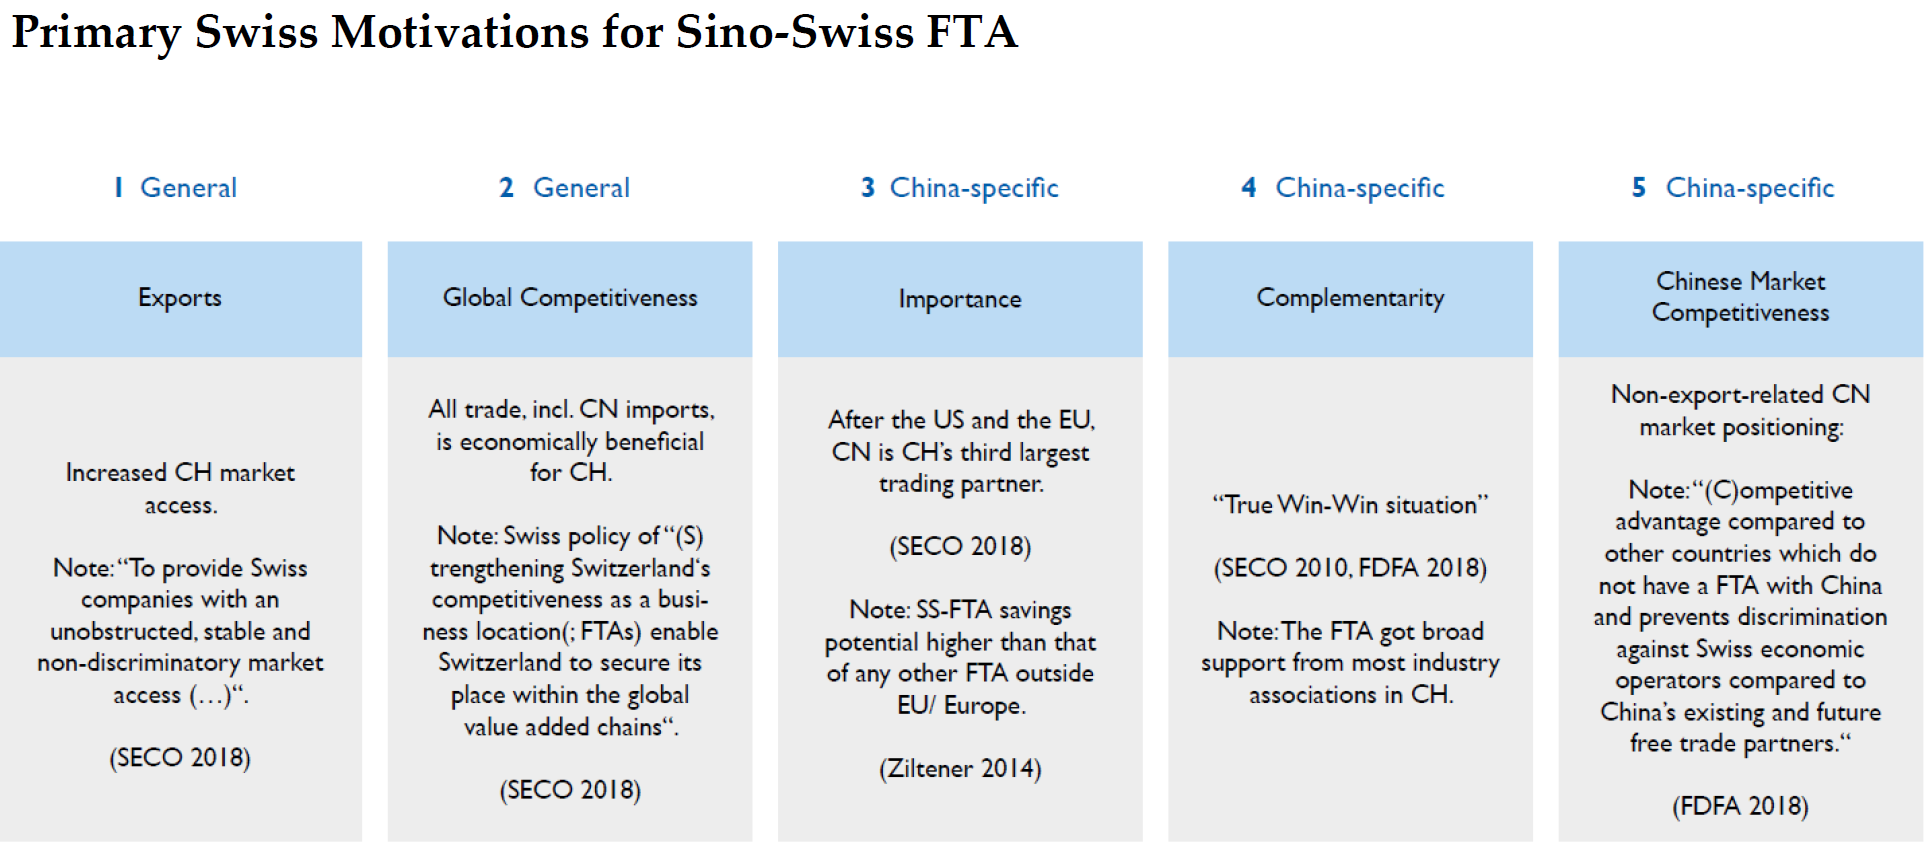
\includegraphics[width=0.9\textwidth]{Pictures/swiss_motivations.png}
\end{figure}


\paragraph{Why China needs Switzerland}

\begin{itemize}
    \item An entry point to European market
    \item A signal to Europe and the west advanced economies
    \item An entry point to the global stage via international organizations
    \item A neutral and friendly country
    \item A balance with Europe and the US
\end{itemize}


\paragraph{Why Switzerland needs China}

\begin{itemize}
    \item A huge and competitive market
    \item Engagement in an emerging power in the global stage
    \item A balance with Wurope and the US
    \item A "client" that Switzerland has been selling its neutrality service to
\end{itemize}

\paragraph{Chinese Strategy: three principle for cooperation}

China has been investing heavily in education, research and innovation for years
and shares a great deal of knowledge in fields including finance, science,
culture and environment protection. It is these areas especially that Switzerland
wishes to cooperate with the PRC, which is listed as a priority country in
Switzerland's Foreign Policy Strategy 2020-23. Three fundamental principles
underpin Switzerland's cooperation with China. These apply to bilateral relations,
multilateral cooperation and coordination in Switzerland.

\begin{itemize}
    \item Switzerland wishes to pursue an independent policy on China and defend
        its long-term interests and fundamental values. It will seek to do this
        through constructively critical dialogue wich Chinese representatves
        in the diverse areas of Swiss-China relations where there is an
        opportunity to engage on the issues.
    \item The Federal Council advocates the integration of China in the liberal
        international order and will seek to coordinate more closely with
        like-minded partners.
    \item Finally, it persues a balanced, coherent and coordinated approach
        to China that encourages exchanges with Parliament, the cantons,
        academia, the private sector and civil society
\end{itemize}

"Pioneering spirit and pragmatism, in addition to a strong stance in the
defence of Swiss interests and values, have moulded Switzerland's policy
on China for seventy years. They will continue to do so." - Ignazio Cassis


\subsection{Competence of the two nations}

\begin{figure}[H]
    \centering
    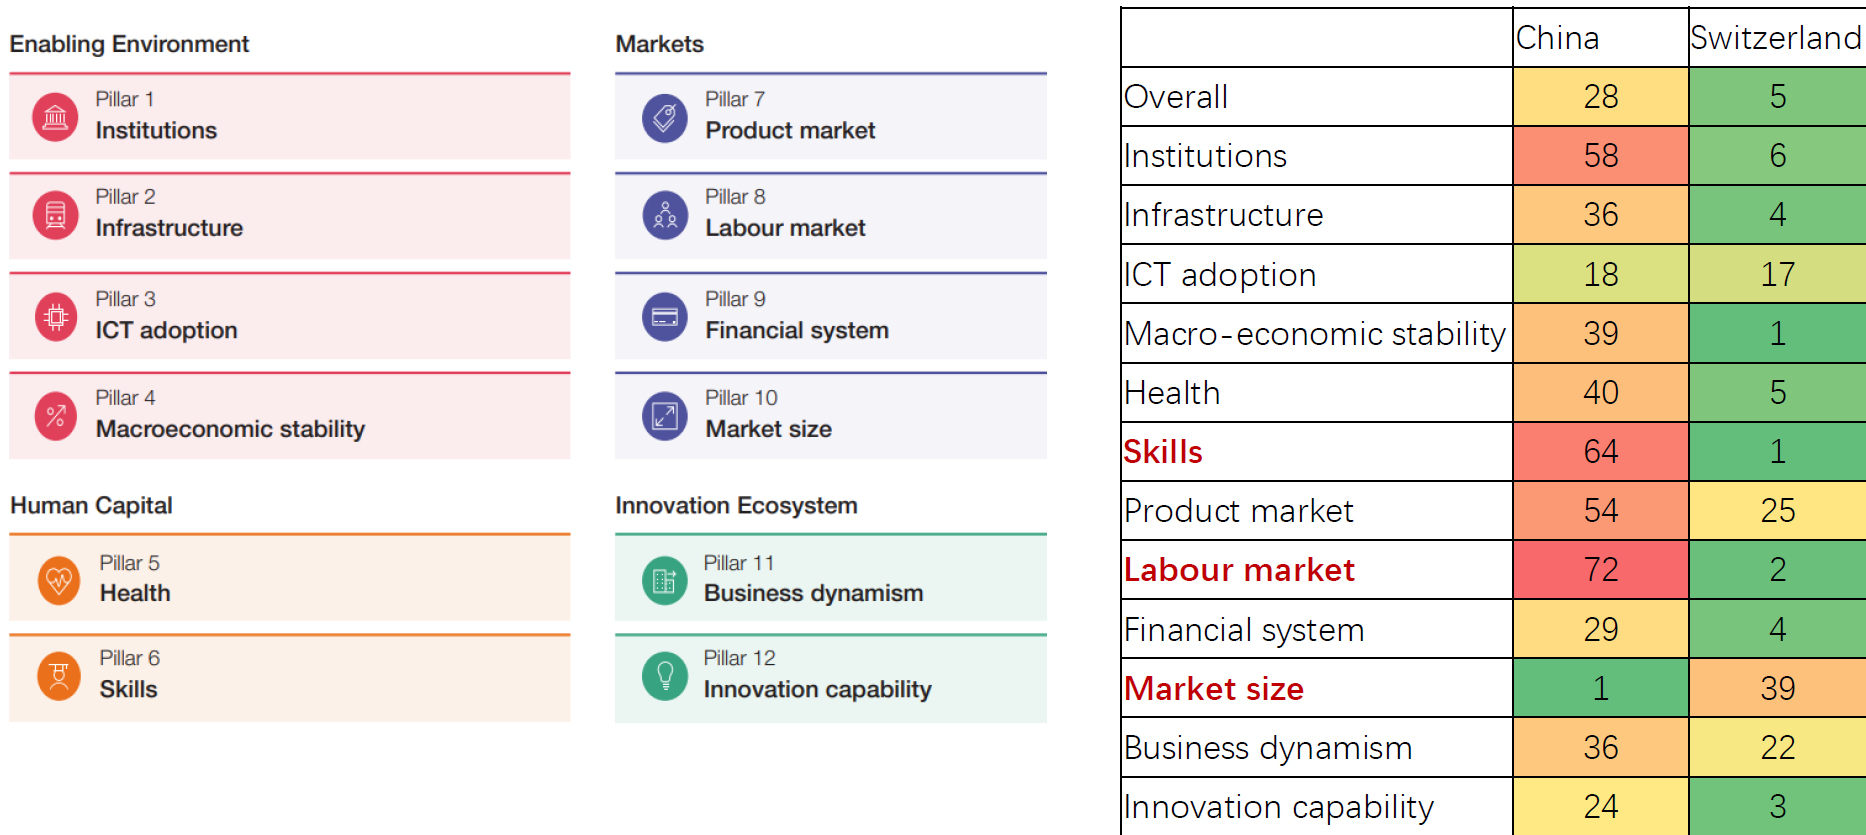
\includegraphics[width=0.9\textwidth]{Pictures/global_competitiveness_index.png}
    \caption{Global Competitiveness Index}
\end{figure}

\begin{figure}[H]
    \centering
    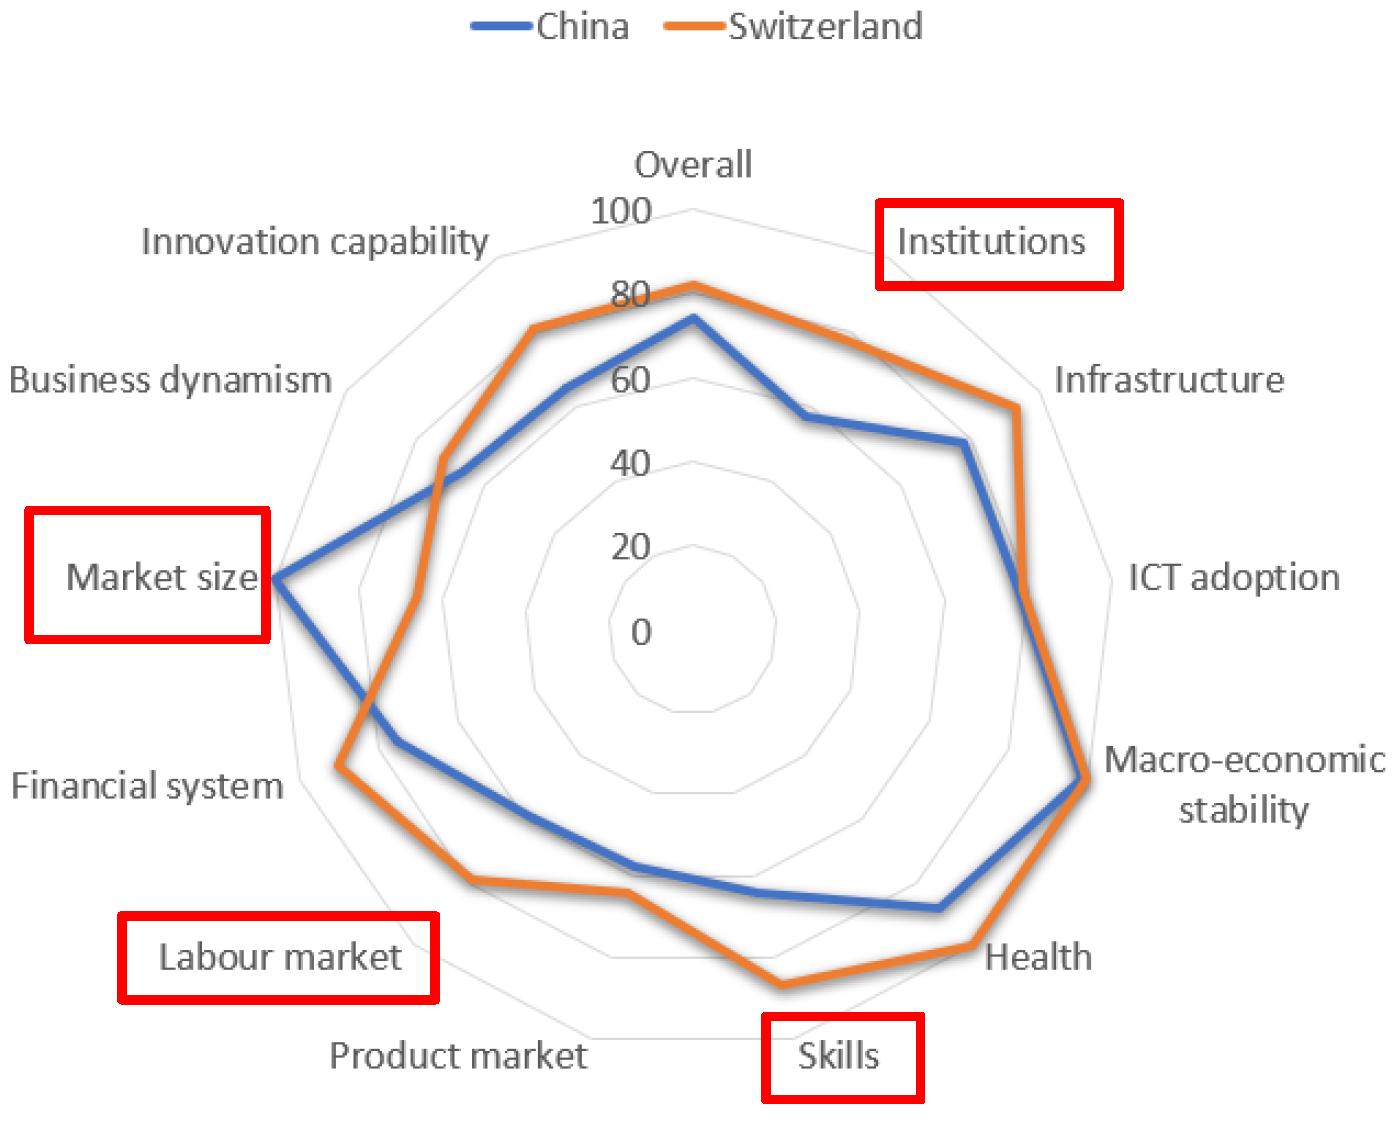
\includegraphics[width=0.5\textwidth]{Pictures/china_switzerland_wef.png}
\end{figure}

Switzerland has been innovation leader for the last 10 years.

\paragraph{Strengths}

\begin{itemize}
    \item G\uproman{2} strengths of China are found in six of the seven
        G\uproman{2} pillars, and mostly on the innovation output side
        of the G\uproman{2}, which captures countries' innovation results.
    \item Several of these strengths are in knowledge and technology outputs,
        the best ranked G\uproman{2} pillar for China. Here the country's
        strengths are sub-pillar knowledge creation and knowledge impact
        and indicators Patents by origin, Utility modely by origin, Labor
        productivity growth, and Hightech exports. In all of these indicators,
        China is world leader this year.
    \item In Creative outputs, China's strengths are sub-pillar Intengible
        assets and indicators Trademarks by origin, Industrial designs by
        origin, and Creative goods exports. In all of these areas, China ranks
        first in the world.
    \item On the innovation input side, China's strengths are found in four
        areas:
        \begin{itemize}
            \item In Human capital and research, an important G\uproman{2}
                strength is indicator Quality of universities, where China is
                placed 3rd worldwide, after the US and the UK.
            \item In Business sophistication, China's strength are indicators
                Firms offering formal training , R\&D financed by business,
                and Hightech imports.
            \item In Market sophistication, relative strengths are sub-pillar
                Trade, competition and market scale and indicator
                Domestic market scale, where China positions 1st globally.
            \item In Infrastructure, China's strength is indicator Gross capital
                formation.
        \end{itemize}
\end{itemize}

\paragraph{Weaknesses}

\begin{itemize}
    \item China's weaknesses in the G\uproman{2} are found in all G\uproman{2}
        pillars, except for knowledge and technology outputs.
    \item Most of these weaknesses are found on the innovation input side of
        the G\uproman{2}, which captures the investment that economies
        make to produce more and better innovations.
    \item In Institutions, China's weaknesses are sub-pillar Regulatory
        environment and its indicator Cost of redundancy dismissal.
    \item In Human capital and research, relative weaknesses are sup-pillar
        Tertiary education and indicator Tertiary inbound mobility.
    \item In Infrastructure, China presents relative weaknesses in two
        indicators within the area Ecological sustainability - GDP per unit
        of energy use and environmental performance.
    \item Indicator Microfinance gross loans in a relative G\uproman{2}
        weakness in Market sophistication.
    \item In Business sophistication, indicators R\&D financed by abroad
        and FDI inflows are G\uproman{2} weaknesses for China.
    \item Three relative weaknesses are found in Creative outputs in indicators
        National feature films, Printing and other media, and Wikipedia edits.
\end{itemize}

\subsection{Swiss startups and innovation}

471 ETH spin-offs since 1996 (93\% 5-Year survival ratio), 41 acquired or went IPO.

The ETH Domain under the Swiss Confederation, which includes 2 federal universities
and 4 federal institutions, forms the backbone of Swiss scientific and
technological innovation, incubating 60-100 Hightech companies each year, with
ETH Zürich being the largest institution in the domain.

\begin{figure}[h]
    \centering
    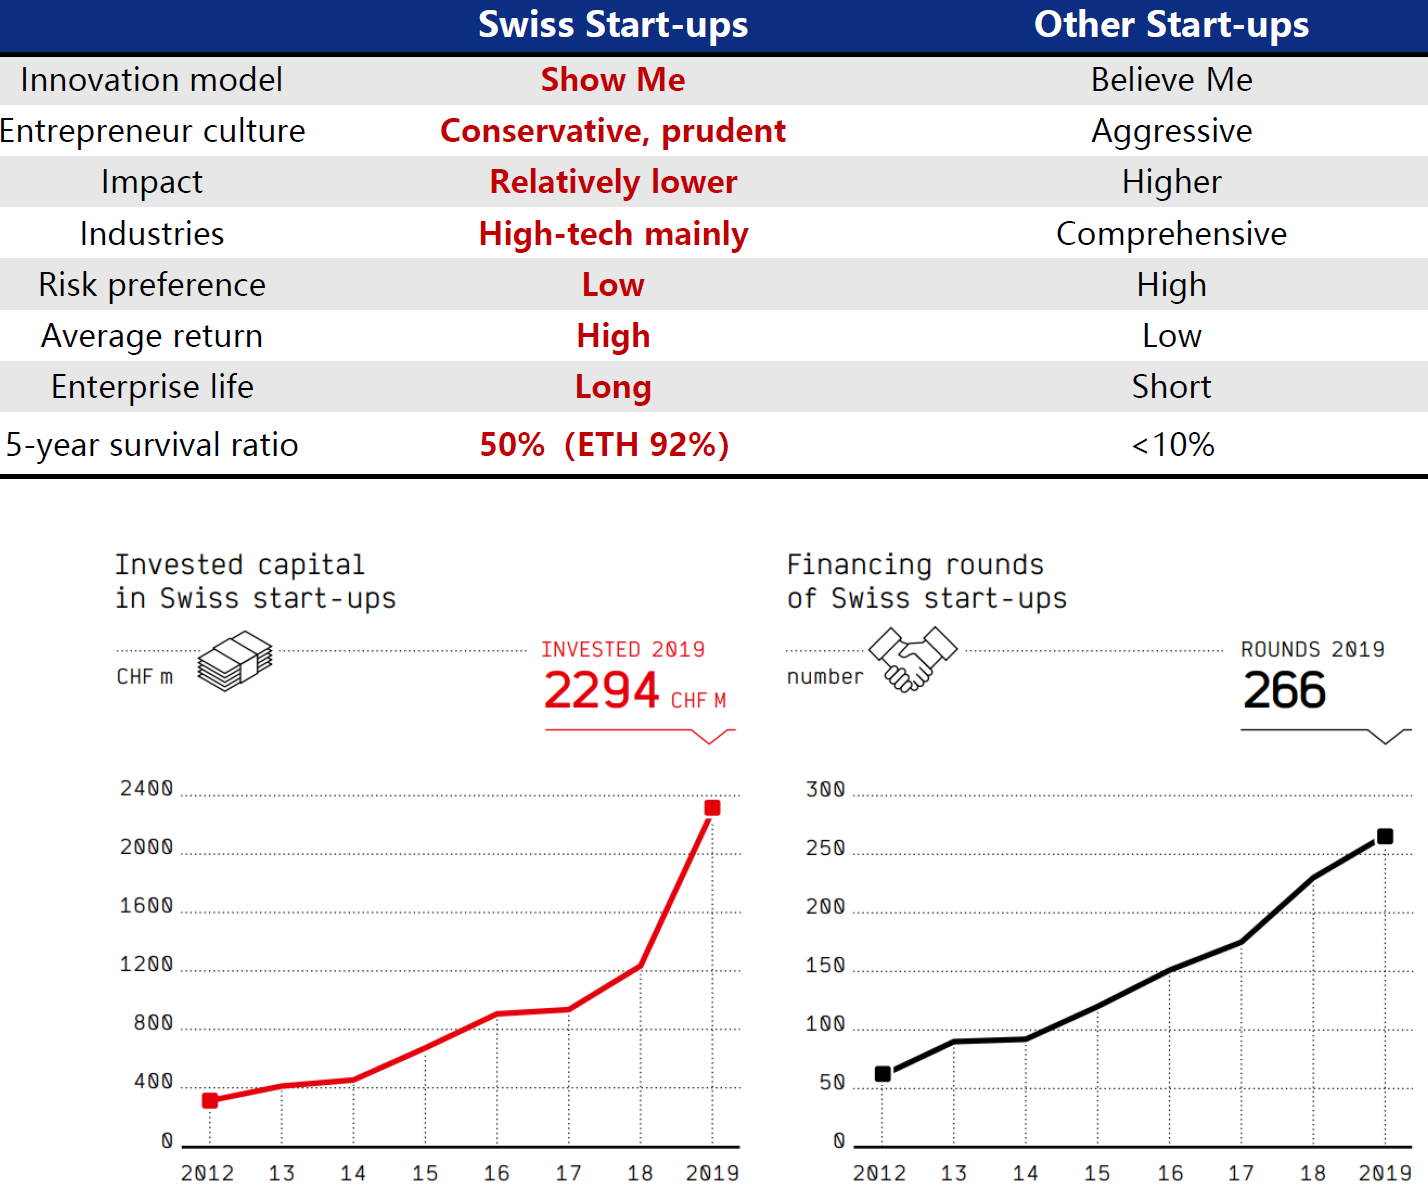
\includegraphics[width=0.7\textwidth]{Pictures/swiss_starups.png}
\end{figure}

Life sciences industry (including biotechnology, medical devices, health
information technology, eth.) as a traditional advantage industry remains
stable. The information and communications technology industry has risen
rapidly in recent years, with a significant growth rate, and the amount
of venture capital investment doubled in 2019.

\vspace{1\baselineskip}

From 2012 to 2018, the average amount of Swiss startup financing increased
by 26\% per year, reaching nearly 8.7 billion yuan in 2018, equivalent to
four times the amount of venture capital in 2012, and an average of 42 million
yuan per finanfing transaction.

Most Projects are very easy to get seed round funding and funds after the
A round, but the intermediate funding (between 2 million and 10 million
Swiss francs) is very difficult to obtain, which provides an excellent
opportunity for Chinese capital to cut in.

\begin{figure}[H]
    \centering
    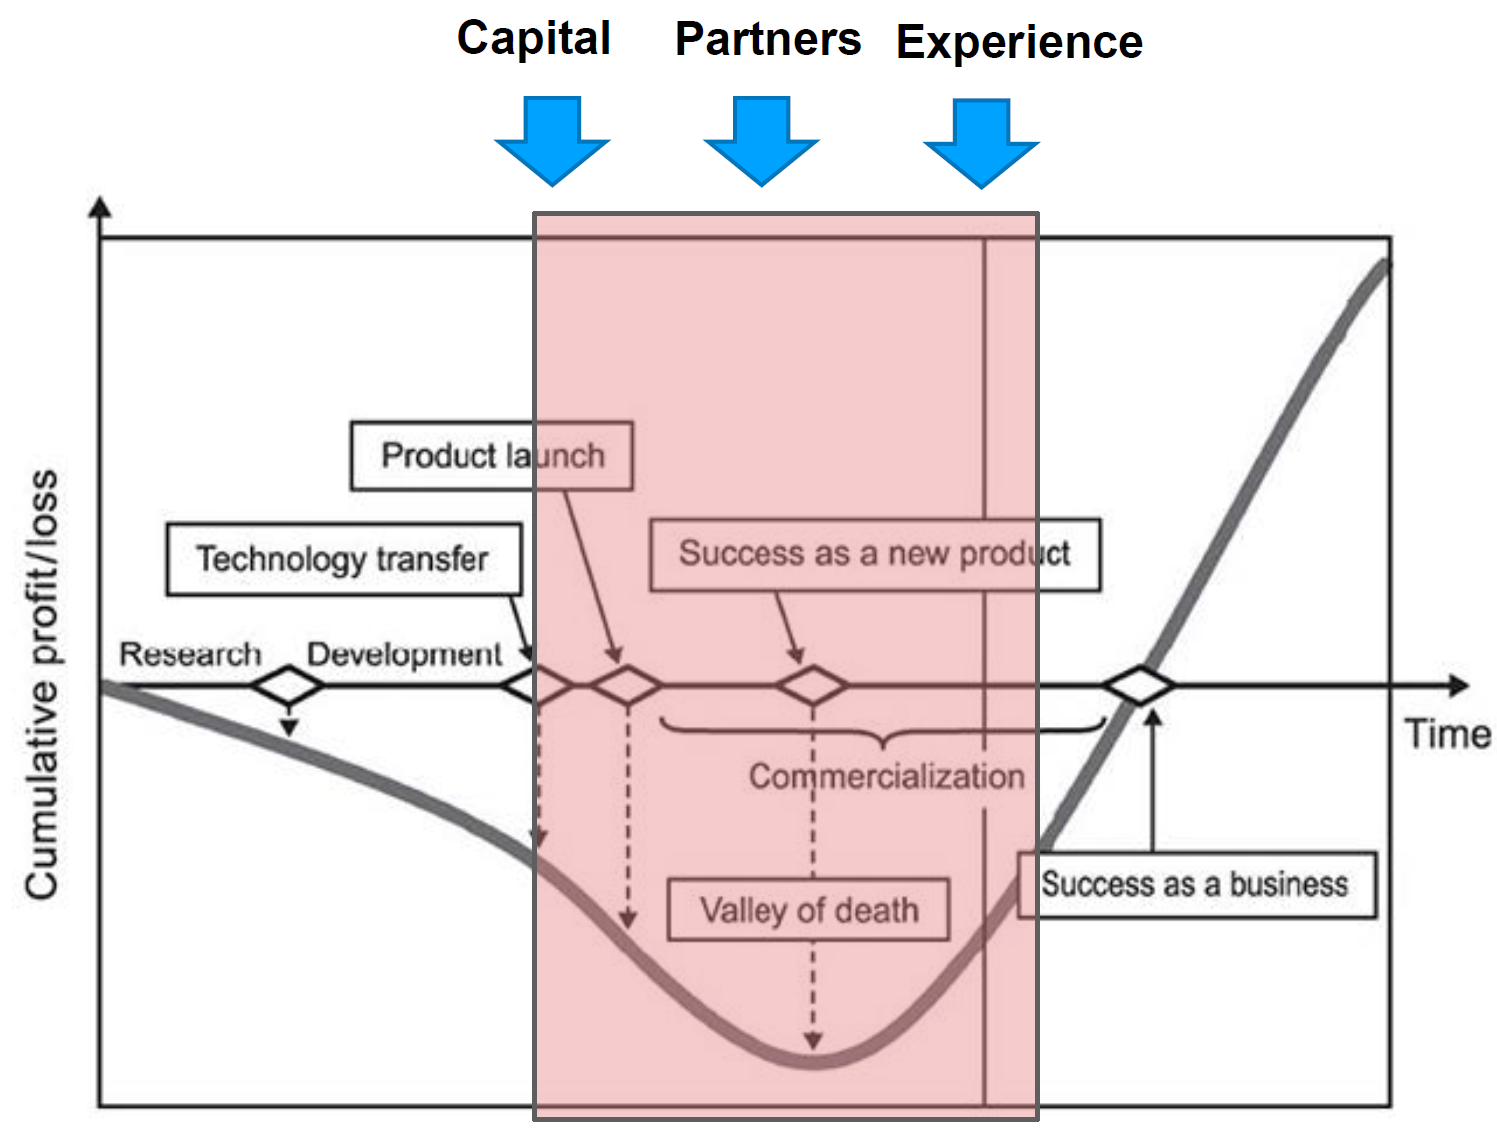
\includegraphics[width=0.45\textwidth]{Pictures/startup_lifecycle.png}
    \hspace{10pt}
    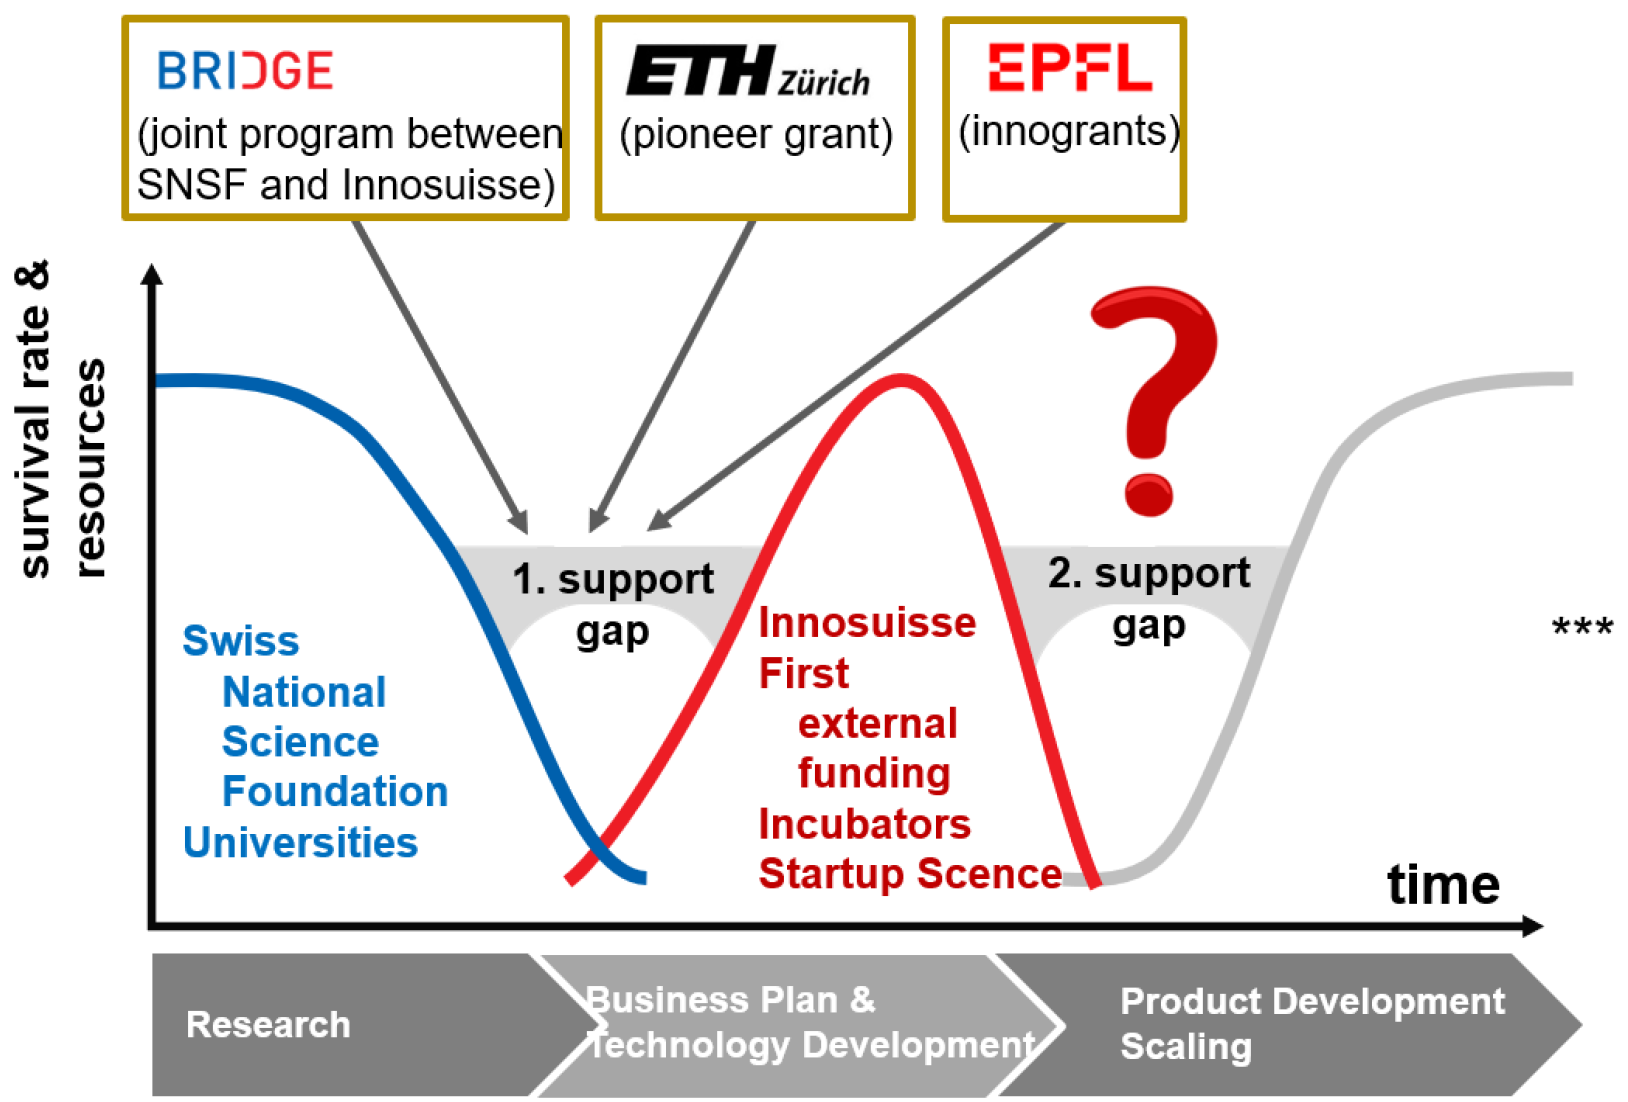
\includegraphics[width=0.45\textwidth]{Pictures/startup_lifecycle_2.png}
\end{figure}

\subsection{Chinese startups and innovation}

China's spending on research and development in science and technology,
surged ten-fold since 2000, while the US spending grew a modest 39\% in the
same period.

The chinese intellectual property protections grew over time just as in the
US just with a time shift of approximately 100-200 years.

\vspace{1\baselineskip}

Innovation refers ot the ability to produce new economic value through the
creation or improvement of products or business services. It can take many
forms. At one end of the spectrum is transformational innovation - something
that fundamentally alters a market or an industry. Often, but not always, it
is based on scientific research. But innovation can also be incremental - a
modification or enhancement to an exciting product or service that improves
its market position and increases its economic value.

\vspace{1\baselineskip}

China has advancced far beyond the mere copying of Western products or
technologies and now excels at incremental innovation. It still lags the US,
Europe, and Japan in transformational, science-based innovation, but with
a sustained policy focus and investment by its government and the leverage
provided by a massive domestic market, transformational innovation can also
be expected to advance.

\vspace{1\baselineskip}

Advances are clear at the national level, in fields such as supercomputing,
quantum communications, space, and robotics. In the private sector,
advances can best be seen in mobile commerve, where China currently leads the
world. While the innovations driving China's commercial success are mostly
incremental, they are increasingly enabled by investment in artificial
intelligence (AI). Outside of mobile commerce - in fields such as semiconductors,
software, commercial aircraft, and life sciences - China's advance is more
uneven. Even in those sectors, however, sustained investment is likely to
bring change.

\begin{figure}[H]
    \centering
    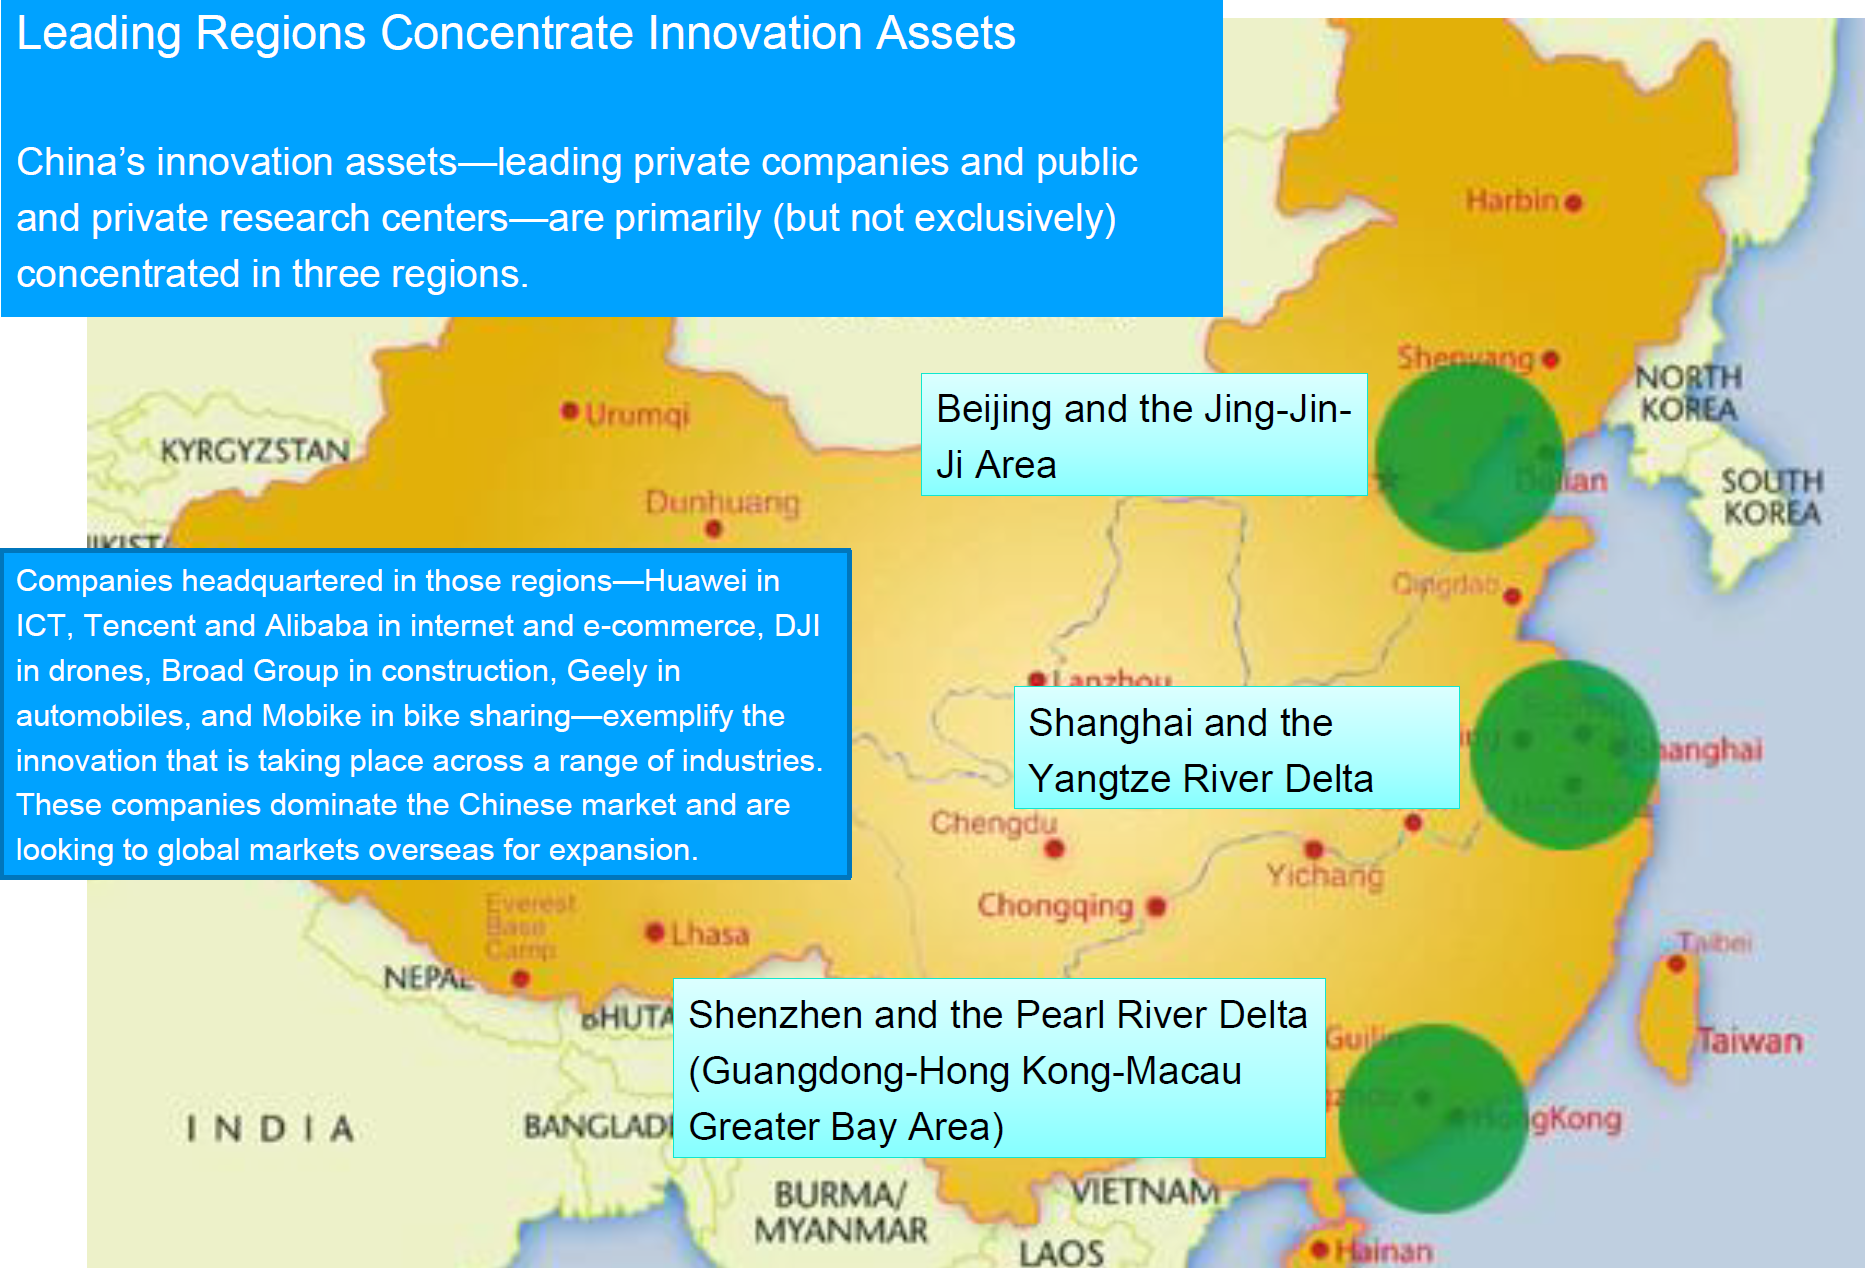
\includegraphics[width=0.65\textwidth]{Pictures/china_innovationhubs.png}
\end{figure}

China also has an increasingly robust starup scene, with a rapidly growing number
of incubators and accelerators. Many are sponsored by provincial and city
governments, offering benefits such as grants or free rent. It is not clear,
however, whether their rapid expansion reflects a similar scale of innovation,
or whether it constitutes a bubble.

\vspace{1\baselineskip}

There is also growing private investment in startups, by large companies such as
Tencent, Alibaba, and Baidu, and through an array of venture capital and private
equity firms. Reflecting the scale of this activity, in 2016 China let Asia in
the production of unicorns (companies with valuations of \$1 billion or more)
with 37; the country with the next largest number was India with 8. Internet
companies are receiving more than half of China's venture deal flow, and of
China's 46 unicorns in 2017, nearly half are backed by China's largest
internet companies.

\vspace{1\baselineskip}

Still, China's startup support ecosystem remains a work in progress. Venture
investors often look to monetize their investments quickly, reinforcing
tendencies in their portfolio companies to go for short-term gains instead
of transformational leaps (an area in which Silicon Valley excels). Most
Chinese universities are also behind the curve when its comes to programs that
generate and support Entrepreneur-led startups.

\vspace{1\baselineskip}

Not a lot of funding goes to early start-ups. Mainly the government invests
in companies which are before the IPO.

\vspace{1\baselineskip}

The ideology is that if your company fails, you disappoint the country becasue
the government invested in your company.

\vspace{1\baselineskip}

Despite several booms and busts in China's short venture capital history
(the 'capital spring' of 2014-2015 gave way to the 'capital winter' of 2016,
which then turned into the 'harvest year' of 2017), the number of private
venture capital institutions has grown from 10 in 1995 to 500 in 2005 and
5'000 in 2015. The composition of venture capital sources has changed over time.
Angel investments became abundant in 2014-2015, as a large number of wealthy
individuals joined the VC fray. With the tightening in 2016, more start-ups
turned to the newly established Third New Board for financing.

\paragraph{The 13th Five Year Plan}

Guiding government strategy for the 2016-2020 period, the 13th Five Year Plan
prioritizes indigenous innovation, the achievement of technological self-sufficiency,
the control of standards, and an expanded government role in the market. The
industries it prioritizes overlap with those targeted in Made in China 2025.
$\Rightarrow$ The 14th Five Year Plan (2021-2025)

\paragraph{Made in China 2025}

Made in China 2025 (MIC 2025) is an industrial policy designed to advance
China's global leadership in manufacturing by promoting indigenous innovation,
domestic brands, domestic standards, domestic production, the control of data.
Its scope reasserts the government's role in ventral economic planning in ways
that favor domestic companies over foreign ones in strategically selected sectors.
One of its many objecitves is the development of national corporate champions
that will one day become global market leaders. It does this in part by setting
global sales and market share targets for Chinese products, backed by directed
government resources. These resources can be used to fund foreign technology
acquisitions, among other purposes.

\paragraph{National Innovation-Driven Development Strategy Outline}

Products by the Central Committee of the Communist Party and the State Council
in 2016, the Outline lays out China's science and technology plans and policies,
promoting objectives similar to those of MIC 2025.

\begin{figure}[H]
    \centering
    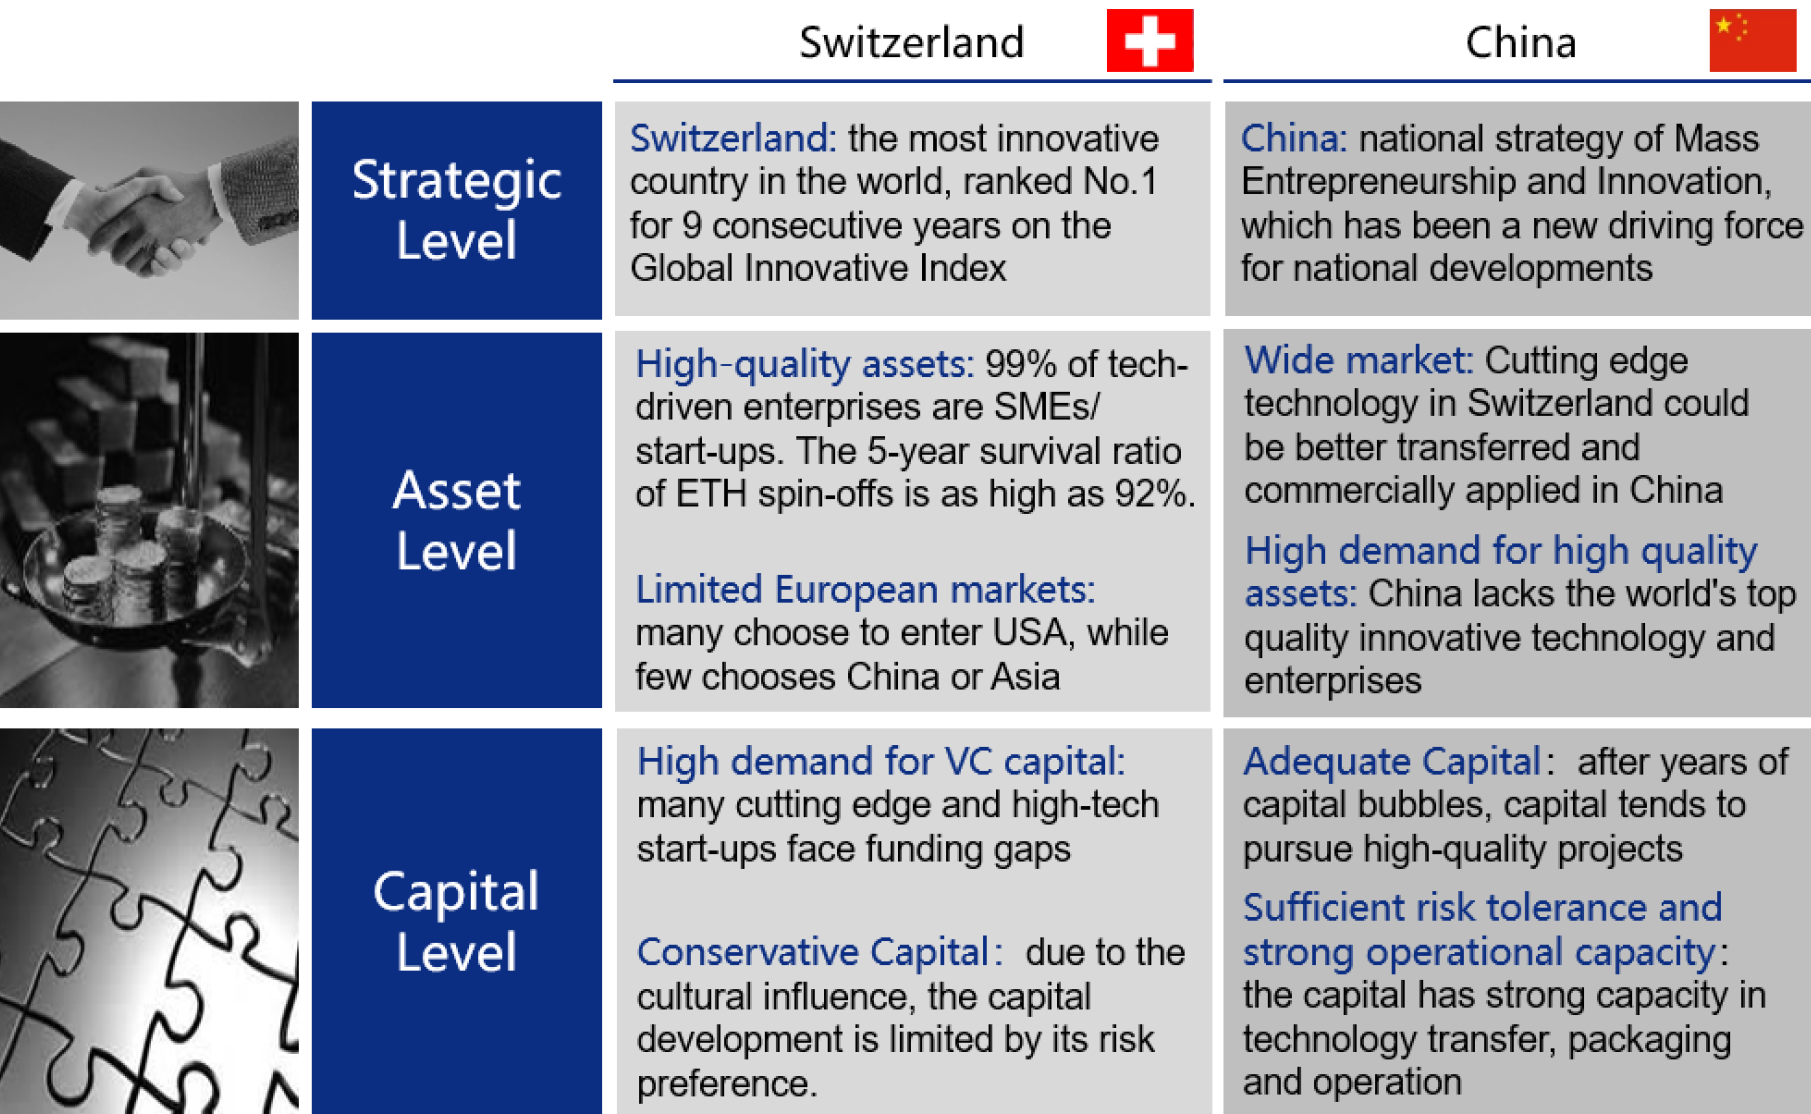
\includegraphics[width=0.7\textwidth]{Pictures/When_bottom_up_meets_top_down.png}
    \caption{When bottom-up meets top-down}
\end{figure}


\subsection{Opportunities}

See lecture Slides.\footnote{\url{https://xyotta.com/cfiles/1233}}

\vspace{1\baselineskip}

China's consumption growth over the next 15 years might be comparable with
that of the US and western Europe.

\begin{itemize}
    \item Wealth management
    \item Discretionary consumption
    \item Health
    \item E-commerce
    \item FinTech
\end{itemize}




